
\section*{Fair Policies (Deadline 2: 19 November)}

\subsubsection*{Sensitive varaibles}
We do not want to discriminate with regards to gender, that is, we want our choice of action to be independent of this variable. 
Income is another variable we could have considered, but to simplify, we will choose gender as our sensitive variable $z$. 


\subsubsection*{Concepts of fairness}
We will look at the concept of fairness as independence. 
Our action $a$ is independent of a variable $z$ if $\mathbb{P}_{\mu}^{\pi}(a|z) = \mathbb{P}_{\mu}^{\pi}(a)$. 
Furthermore, given a response $y$, we can either calibrate or balance the policy with respect to the sensitive variable.  
We will choose the latter, such that the action $a$ is independent of $z$ given the true outcome $y$. 
This is according to the definition of balance (4.3.2):
\begin{align*}
    \mathbb{P}_{\mu}^{\pi}(a|y,z) = \mathbb{P}_{\mu}^{\pi}(a|y) \quad \forall y,z\
\end{align*}
 
\subsubsection*{Measures of fairness}
We need a metric to measure fairness. We will use
\begin{align*}
    F_{\text{balance}}(\mu, \pi) := \sum_{y,z,a}| \mathbb{P}_{\mu}^{\pi}(a|y,z) = \mathbb{P}_{\mu}^{\pi}(a|y)|^2
\end{align*}
To estimate $\mathbb{P}(a_i|y_j,z)$ and $\mathbb{P}(a_i|y_j)$ for $i \in \{\text{No vaccine, vaccine 1, vaccine 2, vaccine 3}\}$ and $j \in \{\text{Presence of critical symptom, Not presence of critical symptom}.\}$ we can use the rate we obtain after running the policy on a simulated population. 
    
\subsubsection*{Tuning a policy to be fair}
Increasing the degree of fairness measured by the fairness-metric, may result in a loss in utility. 
To balance utility and fariness we intriducte the value: 
\begin{align*}
    V(\lambda, \mu, \pi) = (1-\lambda)U(\mu, \pi) - \lambda F(\mu, \pi)
\end{align*}
where $\lambda$ is a parameter that needs to be tuned. 
To find the optimal tradeoff, we can use stochastic gradient descent. 
We have not managed to complete this task. 

The optimization task above is unconstrained with respect to the amount of unfairness. 
However, it might be the case that we can only allow a certain amount of fairness, say $\epsilon$. 
The problem would then be 
\begin{align*}
    \text{max}_{\pi} U(\pi,\mu) \text{ s.t } F(\pi,\mu) < \epsilon
\end{align*}



\subsubsection*{Bias in the data collection}
\textcolor{red}{TODO: describe bias in fairness}
\verbatiminput{../src/outputs/gender_average_100_runs.txt}

\begin{figure}
    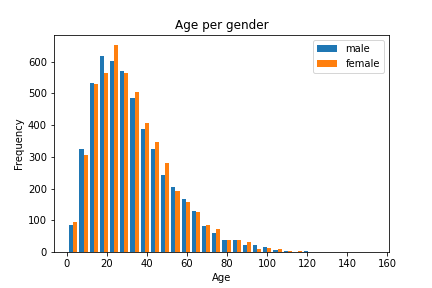
\includegraphics[width=0.6\textwidth]{../src/figures/age_per_gender.png} 
    \includegraphics[width=0.5\textwidth]{../src/figures/age_per_gender_histogram_real.png} 
    \caption{Comparason of distribution of age. Source: SSB 2021}
    \label{Age_comparison}
\end{figure}

\begin{figure}
    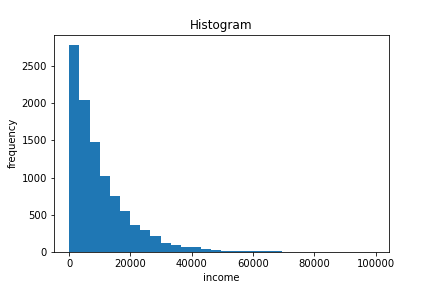
\includegraphics[width=0.6\textwidth]{../src/figures/income_histogram.png} 
    \includegraphics[width=0.5\textwidth]{../src/figures/income_histogram_real.png} 
    \caption{Comparason of distribution of income. Source: US Census Burea 2015}
    \label{Income_comparison}
\end{figure}



\subsubsection*{Results}
\verbatiminput{../src/outputs/default.txt}


\begin{figure}
    \includegraphics[width=0.6\textwidth]{../src/figures/fair_balance_symptom_0.png} 
    \includegraphics[width=0.6\textwidth]{../src/figures/fair_balance_symptom_1.png} 
    \caption{Frequency of action given outcome and sensitive variables}
    \label{Fair_comp}
\end{figure}

\textcolor{red}{TODO: describe Figure \ref{Fair_comp}}

\begin{figure}
    \includegraphics[width=1\textwidth]{../src/figures/fair_F_simulation_histogram.png} 
    \caption{Histogram of unfairness metric balance}
    \label{F_histogram}
\end{figure}

\textcolor{red}{TODO: describe Figure \ref{F_histogram}}


\newpage
\subsection*{START OLD}
\begin{itemize}
    \item \textcolor{blue}{Choose one concept of fairness, e.g. balance of decisions with respect to gender.}
    \begin{itemize}
        \item We will look at the concept of fairness as independence. \\
        Parity: probability of action is independent of the sensitive varaible. 
        \item NEW: We have chosen balance as a fairness criterion. That is, 
        \begin{align*}
            \mathbb{P}(a|y,z) = \mathbb{P}(a|y)
        .\end{align*}
        Here $a$ is the action, $y$ is the outcome and $z$ is a sensitive variable. 
        This means that the action chosen is independent of the sensitive variable given the true outcome $y$. 
        We regard gender to be a sensitive variable. 
        \item \textcolor{red}{QUESTIONS}
        \begin{itemize}
            \item \textcolor{red}{It is contitioned on $y$. What about $x$ is in the feedback?}
        \end{itemize}
        \item We originally chose the fairness criterion equality of opportunity defined as 
        \begin{align*}
            \text{Equality of opportunity} = \text{min} \left( \frac{P(\hat{y} = 1 | z = 1, y = 1)}{P(\hat{y} = 1 | z=0, y=1)} , \frac{P(\hat{y} = 1 | z = 0, y = 1)}{P(\hat{y} = 1 | z=1, y=1)}\right)
        \end{align*}
        However, we got feedback suggusting this is not a good measure of fairness in this case, since it does not account for the action. 
        We insted were encuraged to use a criteria on the form $P(a|x,?) = P(a|x)$. 
        We would like to get some feedback on what $?$ should be. Is '?' f.ex the sensitive variables?
    \end{itemize}
    \item \textcolor{blue}{How can you measure whether your policy is fair?}
    \begin{itemize}
        \item NEW: We need a metric for measuring the degree of fairness with regards to our policy. 
        To this end we can compare the distribution of $\mathbb{P}(a|y,z)$ and $\mathbb{P}(a|z)$. 
        We can sum the squared difference over all $y, z, a$, i.e
        \begin{align*}
            F_{\text{balance}}(\theta, \pi) \triangleq \sum_{y,z,a} |\mathbb{P}_{\theta}^{\pi} (a|y,z) - \mathbb{P}_{\theta}^{\pi}(a|y)|^2
        \end{align*}  
        \item \textcolor{red}{Questions}
        \begin{itemize}
            \item \textcolor{red}{There are two different setups, which should we choose?}
        \end{itemize}
        \item OLD: Given that $P(a|x,z=1) = P(a|x,z=0)$ is a good criteria, we will calcuate this probablity for all the sensitive variables. If we get values close to 1 we will say that our policy is fair. We would also like to have a treshold where values above the thresold are acceptible.
    \end{itemize}
    \item \textcolor{blue}{How does the original training data affect the fairness of your policy?}
    \begin{itemize}
        \item NEW: TODO
        \item \textcolor{red}{What does this point mean?}
        \item OLD: In the simulator, when data is generated, the people are vaccinated. To measure fainess in the original training data we will then see how vaccines are distributed among the senistive variables. 
    \end{itemize}
    \item \textcolor{blue}{To help you in this part of the project, here is a list of guiding questions.}
    \item \textcolor{blue}{(P1)}
        \begin{itemize}
            \item \textcolor{blue}{Identify sensitive variables.}
            \begin{itemize}
                \item NEW: We view gender as a sensitive variable. 
                \item OLD: One sensitive variable with regards to fairness is gender, because we dont want to discriminate people based on their gender. Another sensitive variable is salary, beacuse we dont want to give people a treatment or vaccine based on their salary. For a variable to be considered sensitive we must belive that the variable should not be taken into account by the policy when it chooses an action. 
            \end{itemize}
            \item \textcolor{blue}{Do the original features already imply some bias in data collection?}
            \begin{itemize}
                \item Here we need to present diagrams of how features are distributed in the population. 
                Perhaps start with gender, income and age?
                \item NEW: TODO: tips from AMG: we must state precisely which features in the data that seems relevant and which irrelevant to us. 
                We are not asked to suggest methods for reducting bias. 
                We must strategically find out if the given data might be biased. How?
                \item \textcolor{red}{Questios:}
                \item OLD: To reduce our bias in our data, we must collect data that represents the whole population, and our data collection should not be based on belives we already have. For example if we want to test if a vaccine increases the probabilty of a symptom given a comorbiditie, we should not only collect data from people with the comobordotie, but also from people without that comorbidite, such that our data reflects our entire population. Also, it is important to collect data with variables that is important for our outcome. For example it could be important to use the location of where people live to predict if a person gets infected with Covid-19. A final convern is the the variables must be logical. For instance, having a variables 'number of male children' does not make sense. It would make more sense to inlude the number of children instead. 
            \end{itemize}
        \end{itemize}
    \item \textcolor{blue}{(P2)}
        \begin{itemize}
            \item \textcolor{blue}{Analyse the data or your decision function with simple statistics such as histograms.}
            \begin{itemize}
                \item NEW: 
                \item OLD: We have plotted histograms of some of the variables.
                The age histogram is unrealisitc. For on thing, the birth rate drops exponentially in recent years. Moreover, after the age of around 25 there is an exponentiall decrease in the survival rate. We see that the age of our data is centered between 20-50 years old, which can be a realistic assumption. One problem os however that there is not that much young people, and we also have some very old people (200 years old) which is not realsitic. We also see that our data is balanced in respect to the genders. When it comes to the income of our data, this also looks to reflect a general population. The distribution look like a pareto distribution. We would have expected the histogram to peak the minimum wage and not at 0. 
                \item OLD: We also bootsrap our data to see if there is big variation, but it doesnt look to be any big variation in the data.
            \end{itemize}
        \end{itemize}
    \item \textcolor{blue}{(P3)}
        \begin{itemize}
            \item \textcolor{blue}{For balance (or calibration), measure the total variation of the action (or outcome) distribution for different outcomes (or actions) when the sensitive variable varies.}
            \begin{itemize}
                \item TODO: programming
            \end{itemize}
        \end{itemize}
    \item \textcolor{blue}{(P4)}
        \begin{itemize}
            \item \textcolor{blue}{Advanced: Using stochastic gradient descent, find a policy that balances out fairness and utility.}
            \begin{itemize}
                \item TODO: programming
            \end{itemize}
        \end{itemize}
\end{itemize}

\subsection*{FINISHED OLD}
